\usetikzlibrary{arrows.meta}
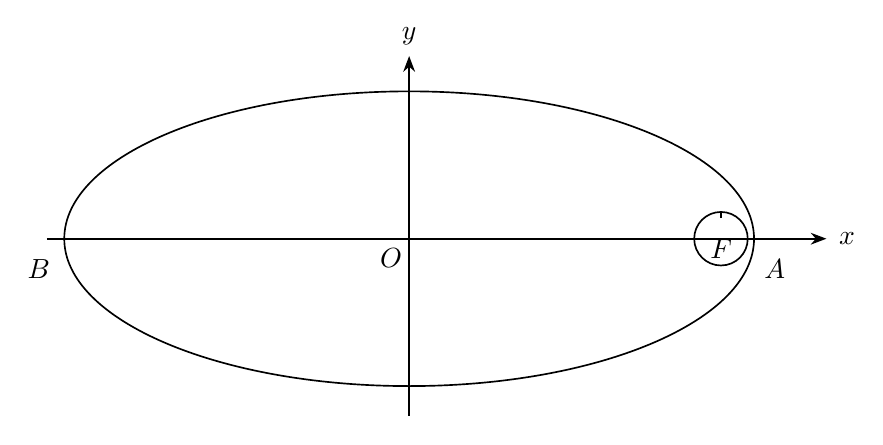
\begin{tikzpicture}[x=1cm,y=1cm,line width=.6pt,font=\normalsize,>=Stealth]
\coordinate (O) at (0,0);
\coordinate (A) at (4.38,0);
\coordinate (B) at (-4.38,0);
\coordinate (F) at (3.96,0);
\draw[->] (-4.6,0)--(5.3,0);
\draw[->] (0,-2.25)--(0,2.32);
\draw (O) ellipse[x radius=4.38,y radius=1.871577];
\draw (F) circle[radius=0.34];
\draw[line width=.4pt] (3.96,0.26)--(3.96,0.33);
\node[anchor=north east,inner sep=0pt] at (-0.08,-0.12) {$O$};
\node[anchor=north west,inner sep=0pt] at (4.5,-0.25) {$A$};
\node[anchor=north east,inner sep=0pt] at (-4.55,-0.25) {$B$};
\node[anchor=north,inner sep=0pt,xshift=.1pt,yshift=-.15pt] at (F) {$F$};
\node[anchor=west,inner sep=0pt] at (5.45,0) {$x$};
\node[anchor=south,inner sep=0pt] at (0,2.45) {$y$};
\end{tikzpicture}
